\documentclass{article}

\usepackage{graphicx} % Required for inserting images
\usepackage{geometry}
\usepackage{float}
\usepackage{tabularray}
\usepackage{listings}
\usepackage{colortbl}
\usepackage[table]{xcolor}

\begin{document}
\setlength{\parindent}{20pt}
\begin{titlepage}
    \centering
    \vspace*{1cm}

    
\includegraphics[width=0.4\textwidth]{Images/dei_thumb.png} % Replace with your university logo

    \vspace{1.5cm}
    {\LARGE \textbf{Teste Dinâmico de Software} \par}
   
    

    \vspace{2.5cm}
    \textbf{Mestrado em Engenharia Informática} \\
    \textbf{Qualidade e Confiabilidade de Software 2023/2024} \\
    \vspace{0.5cm} 
    \textbf{Versão do Documento: 1.0} \\
    \vspace{3cm}
    \begin{tabular}{ll}
        \textbf{Bruno Sequeira} & 2020235721, brunosequeira@student.dei.uc.pt \\
        \textbf{Rui Santos} & 2020225542, rpsantos@student.dei.uc.pt
        
      

    \end{tabular}\\
    \vspace{1.5cm} 
    \textbf{Universidade de Coimbra}

    \date{}

    \vfill

\end{titlepage}
   

\clearpage
\tableofcontents
\clearpage
\listoffigures
\listoftables
\clearpage


\section{Introdução}
\texttt{}\par Este projeto consiste no desenvolvimento de um plano de teste de software de modo a testar, avaliar e testar um software implementado por outros desenvolvedores.\\ 

\texttt{}\par O principal objetivo é identificar e selecionar corretamente abordagens de testes dinâmicoss, tendo em conta testes de White Box e o que este conceitos pode concluir ao executar um plano de teste de software.

\texttt{}\par  Tal como referido acima, escolhemos dois produtos de software, que são os seguintes:

\begin{itemize}
    \item \textbf{Jogo do Sudoku}: Este código iré tentar resolver uma tela 9x9 com as regras do sudoku, sendo que a função que irá abordar essa implementação é a \textbf{Solve()}, está irá percorrer posição a posição, usando um algoritmo de back-tracking para no final retornar um boleano com o resultado, sendo que se for true então foi possível a sua realização, sendo possível visualizar o seu resultado. O input é um array bi-dimensional, e o output é a solução deste array.
    \item \textbf{Algoritmo de Dijkstra}: Este software consiste em encontrar os caminhos mais curtos entre vértices consoante as ligações entre eles. O input é a criação de um grafo e escolhendo um vértice como origem. O resultado final é um array com as distâncias entre o ponto de origem com todos os outros vértices.

\end{itemize}
Na secção 2 serão apresentados os aspetos de risco de software a ser testado e potenciais riscos. Na secção 3 serão apresentados os elementos e funcionalidades a serem testados e na secção 4 serão descritos os elementos e funcionalidades que não serão testados, assumindo que estes pontos esão corretos e bem implementados. \\
Na secção 5 será apresentado os planos de testes, na secção 6 serão definidos os critérios de realização do plano de testes. Na secção 7 serão identificados todos os elementos que foram entregues como parte e consequência do plano de testes. Na secção 8 apresentaremos as necessidades específicas para execução dos testes. Na secção 9 a distribuição do trabalho por elemento. E por fim, a secção 10, será apresentado as conclusões para os resultados dos testes, descrevendo os defeitos identificados.

\section{Aspetos de risco do software}
\texttt{}\par Neste trabalho, a seleção criteriosa e a qualidade dos casos de teste assumem um papel crucial, visto que o código em questão foi desenvolvido para fins académicos e pessoais, sem documentação oficial além do código-fonte fornecido. Essa falta de documentação pode dificultar a compreensão inicial do fluxo do programa.

Além disso, a possibilidade de bus no código levanta a necessidade de testes mais rigorosos para garantir a validade dos resultados.

Por outro lado, visto que é apenas um ficheiro Java, a simplicidade do software elimina a preocupação com dependências externas que possam afetar o seu funcionamento.

\section{Elementos e funcionalidades a serem testadas}

\texttt{}\par Para o software encontrado, iremo-nos focar na função \textbf{Solve} e \textbf{Dijkstra}, sendo que estas irão ser analisadas e serão realizados testes do tipo White Box separadamente em cada função, iremos abordar o control flow e o data flow.
\subsection{Elementos}
\texttt{}\par Da função solve iremos também testar as suas variáveis para o data flow. As variáveis são as seguintes:\\
\begin{itemize}
    \item board - (global)
    \item i
    \item j 
    \item num
\end{itemize}

\texttt{}\par Da função Dijkstra iremos também testar as suas variáveis para o data flow. As variáveis são as seguintes:\\
\begin{itemize}
    \item graph - (global)
    \item visited
    \item numVertices
    \item priorityQueue
    \item newDistance
    \item distance
    \item source - (global)
    \item currentVertex
    \item edges
    \item edge
    \item vertices
    \item i 
\end{itemize}
\subsection{Funcionalidades}

\begin{itemize}
    \item Funcionalidade básica: Testes para garantir que o algoritmo funcione corretamente em situações ideais.
    \item Testes para verificar se o algoritmo lida corretamente com casos especiais, como grafos com ciclos negativos, grafos não conectados, ou casos em que o vértice de destino não é alcançável a partir do vértice de origem.
    \item Verificar se as variáveis são manipuladas e transformadas corretamente em cada módulo.
\end{itemize}
\section{Elementos e funcionalidades a não serem testadas}
\texttt{}\par Baseado nas nossas funções, temos alguns elementos e funcionalidades que não terão o nosso foco. 
\subsection{Elementos}
\texttt{}\par Os elementos da função dijkstra são:
\begin{itemize}
    \item printSolution() - Baixa complexidade
    \item distancesV() - Baixa complexidade
    \item addEdge() - 2 linhas de código
    \item getEdges() - 1 linha de código.
\end{itemize}

\texttt{}\par O elementos da função Solve é:
\begin{itemize}
    \item isPossible() - Baixa Complexidade
\end{itemize}
\texttt{}\par Em relação às variáveis, abordaremos todas, pois as que são utilizadas nas funções são usadas nas funções externas.

\subsection{Funcionalidades}

\texttt{}\par Existem algumas funcionalidades que não iremos focar, que são as seguintes.\\
\begin{itemize}
    \item A complexidade do código.
    \item O tempo que leva para o software ser executado.
    \item E as funcionalidades das funções referidas acima.
\end{itemize}
\clearpage
\section{Abordagem dos testes}
\subsection{Testes White Box}
\texttt{}\par Nesta secção estão presentes os testes de White Box para as funções \textbf{Dijkstra()}, do projeto \textit{Algoritmo de Dijkstra}, e  \textbf{Solve()} do projeto \textit{Sudoku}.

As técnicas de White Box analisam as estruturas internas, as estruturas de dados usadas, o design interno, a estrutura do código e o funcionamento do software, em vez de apenas a funcionalidade como no teste de caixa preta.


Esta abordagem faz a testagem por partes, ou seja, aos detalhes na implementação do código em análise e foca-se nos testes de \textit{Control-Flow}, onde foram analisados todos os caminhos independentes e implementados casos de testes para cada um.

\subsubsection{Control Flow}
\quad O fluxo de controlo é fundamental no contexto do teste de software. Este se refere à maneira como o controlo é direcionado ou manipulado dentro de um programa ou sistema durante a execução dos testes. O objetivo principal do fluxo de controlo nos testes de software é garantir que todas as partes do código sejam testadas de maneira adequada e eficiente, identificando falhas e garantindo a qualidade do software.


\texttt{}\par Para realização deste método, iremos apresentar passo a passo, a implementação deste. Projetando o grafo de Control Flow de cada função, determinamos a complexidade ciclomática, analisamos os caminho independentes possíveis e verificamos quais deles são possíveis de serem executados. Com isso, iremos determinar casos de teste para cada um dos caminhos encontrados.
\clearpage
\begin{itemize}
    \item \textbf{Função Dijkstra()}
    
       
    \begin{enumerate}
        
        \item \textbf{Grafo de Control Flow}
    \begin{figure}[H]
    \centering
    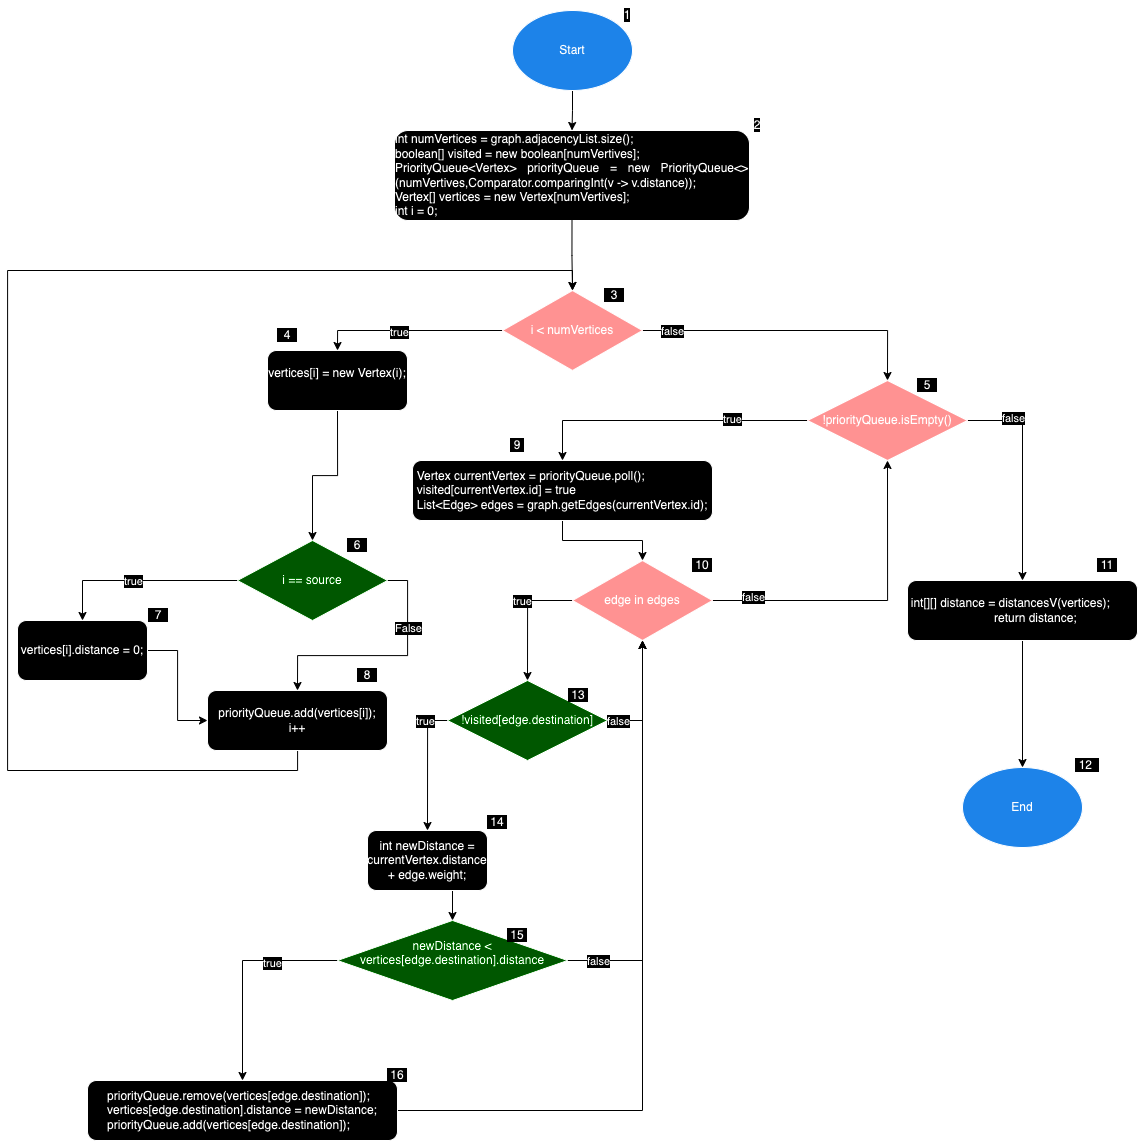
\includegraphics[width=\textwidth]{Images/ControlFlowGraphDijkstra.png}
    \caption{Control Flow - função Dijkstra.} 
    \label{fig:ControlFlow-Dijkstra}

  \end{figure}


  \item \textbf{Complexidade Ciclomática V(G)}
  \quad A complexidade ciclomática é utilizada para determinar o número máximo de caminhos independentes do programa.\\
  \quad A fórmula usada é: \textbf{V(G) = P + 1}.\\

  O \textbf{P} corresponde a nós predicativos.\\

  Nós predicativos são os que têm vários arcos de saída, ou seja, corresponde a condições do programa, tais como, if's, while's e for's.

  \quad Logo, ao analisar a figura de cima, podemos verificar que existem 6 nós predicativos, send o  3  de l es if's (cor verde)  e  3  de l es while's ou for's (cor rosa).

  Portanto a complexidade ciclomática é de 6 + 1 = 7. O que implica que existem no máximo 7 caminhos independentes.
  
  \item \textbf{Caminhos linearmente independentes}\\

  \quad Um caminho linearmente independente é uma sequência de estados de um programa que não pode ser formada combinando outras sequências de estados já testadas, ou seja, é uma sequência única de instruções que representa uma linha de execução distinta no programa.
  Testar caminhos linearmente independentes é importante para garantir uma cobertura abrangente do código.

  Os próximos pontos são os 7 caminhos independentes que encontramos para o código Dijkstra.
  \begin{itemize}
    \item \textbf{P1} = {Start,  2, 3, 5, 11, End}
    \item \textbf{P2} = {Start, 2, 3, 4, 6, 8, 3, 5, 11, End}
    \item \textbf{P3} = {Start, 2, 3, 4, 6, 8, 3, 5, 9, 10, 5, 11, End}
    \item \textbf{P4} = {Start, 2, 3, 4, 6, 7, 8, 3, 5, 9, 10, 5, 11, End}
    \item \textbf{P5} = {Start, 2, 3, 4, 6, 7, 8, 3, 5, 9, 10, 13, 10, 5, 11, End}
    \item \textbf{P6} = {Start, 2, 3, 4, 6, 7, 8, 3, 5, 9, 10, 13, 14, 15, 10, 5, 11, End}
    \item \textbf{P7} = {Start, 2, 3, 4, 6, 7, 8, 3, 5, 9, 10, 13, 14, 15, 16, 10, 5, 11, End}
  \end{itemize}
  NOTA: Start e End correspondem aos estados 1 e 12, respetivamente.

  Destes 7 caminhos linearmente independentes, 2 deles não são executáveis, estes 2 são \textbf{P1} e \textbf{P2}.\\

  \quad Apresentamos agora as razões pelas quais estes não são executáveis são as seguintes: \\
  \begin{itemize}
    \item \textbf{P1} = Neste caso, seria necessário que o grafo não contivesse nenhum elemento, mas para que a funcionalidade da função resulte seria necessário um vértice source, logo o grafo teria de ter pelo menos 1 elemento, só que este iria passar do estado 3 para o estado 4, o que não é o que este caminho deseja. Não sendo possível ser executado.\\
    \item \textbf{P2} = Neste caminho, se o grafo tem de ter pelo menos um elemento, então a fila de vértices é sempre pelo menos um elemento, portanto é impossível a condição do estado 5 ser falsa, visto que no estado 8 é adicionado o elemento na fila. 
  \end{itemize}


  \item \textbf{Casos de teste}\\
  \texttt{}\par Para cada caminho executável iremos apresentar os casos de usos, com o input e o output desejado.
 O input são várias variáveis, o \textit{numVertices} corresponde ao número de vértices que estão presentes no grafo, o \textit{graph} é o grafo que foi criado com o número de vértices anteriormente apresentada. E o \textit{distance} é o que vai conter o output da função chamada que tem como parâmetros o grafo e o vértice de origem para calcular as distâncias.\\

 O output é um array bi-dimensional que contém as distâncias entre o vértice origem com todos o outros vértices que estão presentes no grafo anteriormente criado.\\


\begin{table}[H]
    \centering
    \begin{tabular}{|c|p{7cm}|p{3cm}|} % Ajusta a largura da coluna "Input" para 5cm
    \hline
    \textbf{Caminho} & \textbf{Input} & \textbf{Output Esperado} \\
                        
    \hline
    \textbf{P3} & int numVertices = 1; \newline
                Graph graph = new Graph(numVertices); \newline
                int[][] distance = dijkstra(graph, 1); & 0 - 2147483647  \\
    \hline
    \textbf{P4} & int numVertices = 1;\newline
    Graph graph = new Graph(numVertices);\newline
    int[][] distance = dijkstra(graph, 0); & 0 - 0 \\
    \hline
    \textbf{P5} & int numVertices = 5;\newline
    Graph graph = new Graph(numVertices);\newline
    graph.addEdge(1,2,1);\newline
    graph.addEdge(2,4,5);\newline
    graph.addEdge(2,3,10);\newline
    graph.addEdge(3,4,3);\newline
    int[][] distance = dijkstra(graph, 0); & 0 - 0\newline
    1 - 2147483647\newline
    2 - 2147483647\newline
    3 - 2147483647\newline
    4 - 2147483647   \\
    \hline
    \textbf{P6} & int numVertices = 2;\newline
    Graph graph = new Graph(numVertices);\newline
    graph.addEdge(0, 1, Integer.MAX\_VALUE); \newline
    int[][] distance = dijkstra(graph, 0); & 0 - 0\newline
    1 - 2147483647 \\
    \hline
    \textbf{P7} & int numVertices = 5;\newline
    Graph graph = new Graph(numVertices);\newline
    graph.addEdge(0,2,1);\newline
    graph.addEdge(0,1,10);\newline
    graph.addEdge(2,4,5);\newline
    graph.addEdge(2,3,10);\newline
    graph.addEdge(3,4,3);\newline
    int[][] distance = dijkstra(graph, 0); & 0 - 0\newline
    1 - 10\newline
    2 - 1\newline
    3 - 11\newline
    4 - 6 \\
    \hline
   
    \end{tabular}
    \caption{Casos de teste para os caminhos independentes do Dijkstra.}
    \label{tab:tabela_exemplo}
\end{table}
\clearpage

  
  

\end{enumerate}
\item \textbf{Sudoku}
\begin{enumerate}
    \item \textbf{Grafo de Control Flow}\\
    \begin{figure}[H]
        \centering
        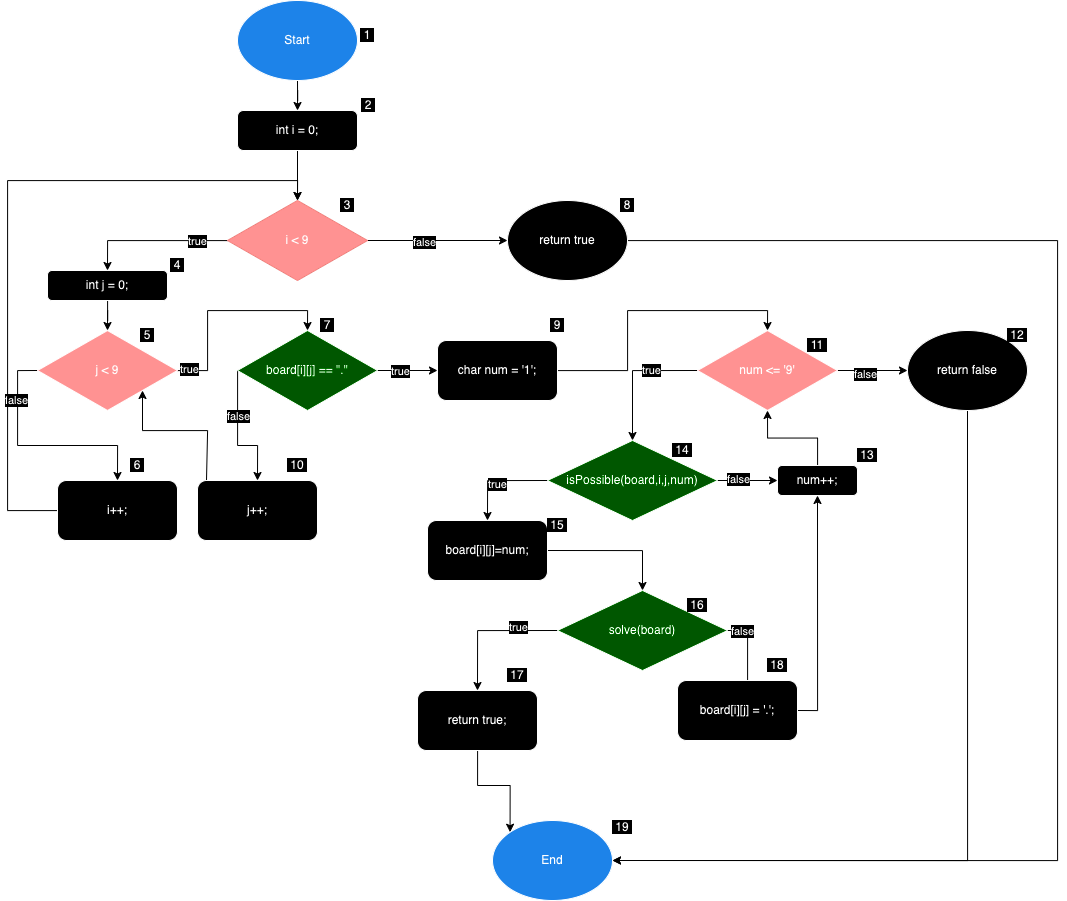
\includegraphics[width=\textwidth]{Images/ControlFlowSudoku.png}
        \caption{Control Flow - função Solve.} 
        \label{fig:ControlFlow-Sudoku}
    \end{figure}
    \item \textbf{Complexidade Ciclomática V(G)}\\
    
    \quad A complexidade ciclomática é utilizada para determinar o número máximo de caminhos independentes do programa.\\
    \quad A fórmula usada é: \textbf{V(G) = P + 1}.\\
  
    O \textbf{P} corresponde a nós predicativos.\\
  
    Nós predicativos são os que têm vários arcos de saída, ou seja, corresponde a condições do programa, tais como, if's, while's e for's.
  
    \quad Logo, ao analisar a figura de cima, podemos verificar que existem 6 nós predicativos, send o  3  de l es if's (cor verde)  e  3  de l es while's ou for's (cor rosa).
  
    Portanto a complexidade ciclomática é de 6 + 1 = 7. O que implica que existem no máximo 7 caminhos independentes.
    
    \item \textbf{Caminhos linearmente independentes}\\
    \texttt{}\par Testar caminhos linearmente independentes é importante para garantir uma cobertura abrangente do código.

  Os próximos pontos são os 6 caminhos independentes que encontramos para o código Solve do código Sudoku.
  \begin{itemize}
    \item \textbf{P1} = {Start, 2, 3, 5, 8, End}
    \item \textbf{P2} = {Start, 2, 3, 4, 5, 7, 10, 5, 6, 3, 8, End}
    \item \textbf{P3} = {Start, 2, 3, 4, 5, 7, 9, 11, 14, 15, 16, 17, End} 
    \item \textbf{P4} = {Start, 2, 3, 4, 5, 7, 9, 11, 14, 13, 11, 12, End}
    \item \textbf{P5} = {Start, 2, 3, 4, 5, 7, 9, 11, 14, 13, 11, 14, 15, 16, 18, 13, 11, 14, 13, 11, 12, End}
   \item \textbf{P6} = {Start, 2, 3, 4, 5, 7, 10, 5, 6, 3, 4, 5, 7, 10, 5, 7, 9, 11, 14, 13, 11, 14, 15, 16, 17, End}
    \end{itemize}
    
  Destes 6 caminhos linearmente independentes, 1 deles não é executáveis, o \textbf{P1}.

  \quad Apresentamos agora as razões pelas quais estes não são executáveis são as seguintes: \\
  \begin{itemize}
    \item \textbf{P1} = Neste caso, não encontramos nenhum caso de teste para realização deste caminho, visto que a variável \textbf{i} é inicializada por 0, e a condição seguinte é sempre verdadeira, o que torna assim um caminho \textbf{unfeasable}.

  \end{itemize}
    \item \textbf{Casos de teste}\\
    \texttt{}\par Para cada caminho executável iremos apresentar os casos de usos, com o input e o output
desejado.
\quad Apresentamos o número do caminho linearmente independente, com o input neste caso o input é o conteúdo da variável \textbf{board} do código que foi submetido do Sudoku, o output é o resultado esperado. Sendo que sempre que existe uma solução este algoritmo altera o board, mas se não encontrar nenhuma solução este irá apresentar o mesmo board que foi submetido.
\begin{table}[H]
    \centering
    \begin{tabular}{|c|p{7cm}|p{3cm}|} % Ajusta a largura da coluna "Input" para 5cm
    \hline
    \renewcommand{\arraystretch}{1.8}
    \textbf{Caminho} & \textbf{Input - Este input é correspondente à variável board.} & \textbf{Output Esperado} \\
                        
    \hline
    \textbf{P2} &   
        {'5', '3', '4', '6', '7', '8', '9', '1', '2'},\newline
        {'6', '7', '2', '1', '9', '5', '3', '4', '8'},\newline
        {'1', '9', '8', '3', '4', '2', '5', '6', '7'},\newline
        {'8', '5', '9', '7', '6', '1', '4', '2', '3'},\newline
        {'4', '2', '6', '8', '5', '3', '7', '9', '1'},\newline
        {'7', '1', '3', '9', '2', '4', '8', '5', '6'},\newline
        {'9', '6', '1', '5', '3', '7', '2', '8', '4'},\newline
        {'2', '8', '7', '4', '1', '9', '6', '3', '5'},\newline
        {'3', '4', '5', '2', '8', '6', '1', '7', '9'}; & 
    5 3 4 6 7 8 9 1 2 \newline
    6 7 2 1 9 5 3 4 8 \newline
    1 9 8 3 4 2 5 6 7 \newline
    8 5 9 7 6 1 4 2 3 \newline
    4 2 6 8 5 3 7 9 1 \newline
    7 1 3 9 2 4 8 5 6 \newline
    9 6 1 5 3 7 2 8 4 \newline
    2 8 7 4 1 9 6 3 5 \newline
    3 4 5 2 8 6 1 7 9   \\
    \hline
    \textbf{P3} & 
        {'.', '.', '.', '.', '.', '.', '.', '.', '.'},\newline
        {'.', '.', '.', '.', '.', '.', '.', '.', '.'},\newline
        {'.', '.', '.', '.', '.', '.', '.', '.', '.'},\newline
        {'.', '.', '.', '.', '.', '.', '.', '.', '.'},\newline
        {'.', '.', '.', '.', '.', '.', '.', '.', '.'},\newline
        {'.', '.', '.', '.', '.', '.', '.', '.', '.'},\newline
        {'.', '.', '.', '.', '.', '.', '.', '.', '.'},\newline
        {'.', '.', '.', '.', '.', '.', '.', '.', '.'},\newline
        {'.', '.', '.', '.', '.', '.', '.', '.', '.'}; & 1 2 3 4 5 6 7 8 9\newline
    4 5 6 7 8 9 1 2 3\newline
    7 8 9 1 2 3 4 5 6\newline
    2 1 4 3 6 5 8 9 7\newline
    3 6 5 8 9 7 2 1 4 \newline
    8 9 7 2 1 4 3 6 5\newline
    5 3 1 6 4 2 9 7 8\newline
    6 4 2 9 7 8 5 3 1\newline
    9 7 8 5 3 1 6 4 2 \\
    \hline
    \textbf{P4} &  
        {'.', '3', '4', '5', '7', '8', '9', '1', '2'},\newline
        {'6', '7', '2', '1', '9', '5', '3', '4', '8'},\newline
        {'1', '9', '8', '3', '4', '2', '5', '6', '7'},\newline
        {'8', '5', '9', '7', '6', '1', '4', '2', '3'},\newline
        {'4', '2', '6', '8', '5', '3', '7', '9', '1'},\newline
        {'7', '1', '3', '9', '2', '4', '8', '5', '6'},\newline
        {'9', '6', '1', '5', '3', '7', '2', '8', '4'},\newline
        {'2', '8', '7', '4', '1', '9', '6', '3', '5'},\newline
        {'3', '4', '5', '2', '8', '6', '1', '7', '9'}; & 
        . 3 4 5 7 8 9 1 2 \newline
        6 7 2 1 9 5 3 4 8 \newline
        1 9 8 3 4 2 5 6 7 \newline
        8 5 9 7 6 1 4 2 3 \newline
        4 2 6 8 5 3 7 9 1 \newline
        7 1 3 9 2 4 8 5 6 \newline
        9 6 1 5 3 7 2 8 4 \newline
        2 8 7 4 1 9 6 3 5 \newline
        3 4 5 2 8 6 1 7 9   \\
\hline
   
    \textbf{P5} & 
        {'.', '.', '4', '6', '7', '8', '9', '1', '2'},\newline
        {'.', '7', '2', '1', '9', '5', '3', '4', '8'},\newline
        {'1', '9', '8', '3', '4', '.', '5', '6', '7'},\newline
        {'8', '5', '.', '7', '6', '1', '4', '2', '3'},\newline
        {'2', '2', '6', '8', '5', '3', '.', '.', '1'},\newline
        {'7', '1', '3', '9', '2', '4', '8', '5', '6'},\newline
        {'9', '.', '1', '.', '3', '.', '2', '8', '4'},\newline
        {'.', '8', '7', '4', '1', '9', '6', '3', '5'},\newline
        {'3', '4', '5', '2', '.', '6', '1', '7', '9'}; & . . 4 6 7 8 9 1 2 \newline
    . 7 2 1 9 5 3 4 8 \newline
    1 9 8 3 4 . 5 6 7 \newline
    8 5 . 7 6 1 4 2 3 \newline
    2 2 6 8 5 3 . . 1 \newline
    7 1 3 9 2 4 8 5 6 \newline
    9 . 1 . 3 . 2 8 4 \newline
    . 8 7 4 1 9 6 3 5 \newline
    3 4 5 2 . 6 1 7 9 \\
    \hline
    \textbf{P6} & 
        {'5', '3', '4', '6', '7', '8', '9', '1', '2'},\newline
        {'6', '7', '2', '1', '9', '5', '3', '4', '8'},\newline
        {'1', '9', '8', '3', '4', '2', '5', '6', '7'},\newline
        {'8', '5', '9', '7', '6', '1', '4', '2', '3'},\newline
        {'4', '2', '6', '8', '5', '3', '7', '9', '1'},\newline
        {'7', '1', '3', '9', '2', '4', '8', '5', '6'},\newline
        {'9', '6', '1', '5', '3', '7', '2', '8', '4'},\newline
        {'2', '8', '7', '4', '1', '9', '6', '3', '5'},\newline
        {'3', '4', '5', '2', '8', '6', '1', '7', '.'}; &5 3 4 6 7 8 9 1 2 \newline
    6 7 2 1 9 5 3 4 8\newline
    1 9 8 3 4 2 5 6 7\newline
    8 5 9 7 6 1 4 2 3\newline
    4 2 6 8 5 3 7 9 1\newline
    7 1 3 9 2 4 8 5 6\newline
    9 6 1 5 3 7 2 8 4\newline
    2 8 7 4 1 9 6 3 5\newline
    3 4 5 2 8 6 1 7 9\\
    \hline
   
    \end{tabular}
    \caption{Casos de teste para os caminhos independentes do Sudoku.}
    \label{tab:tabela_exemplo}
\end{table}

\end{enumerate}

\end{itemize}
\subsubsection{Data Flow}

\texttt{}\par O teste de Data flow é um processo de coleta de informações sobre como as variáveis fluem os dados no programa. Ele tenta obter informações específicas de cada ponto específico no processo. O teste de fluo de dados tem um grupo de estratégias de teste para examinar o fluxo de controlo de programas, a fim de explorar a sequência de variáveis de acordo com a sequência de eventos. Ele se concentra principalmente nos pontos em que os valores são atribuídos às váriaves e o ponto em que estes são usados.\\

\textbf{Vantagem:}\\
O teste de fluxo de dados é usado para encontrar os seguintes problemas:\\
\begin{itemize}
    \item Encontrar uma variável usada, mas nunca definida.
    \item Encontrar uma variável definida, mas nunca usada.
    \item Encontrar uma variável definida várias vezes antes de ser usada.
\end{itemize}

\textbf{Desvantagem:}\\
O processo é demorado.\\


\texttt{}\par Existem vários tipos de teste de fluxo de dados, tais como All def, All use, All-Du-Paths, sendo que este último é o tipo de teste que iremo-nos focar mais, pois esta técnica apesar de ser mais complexa, é a melhor pois analisa todos os caminhos possíveis de uma definição de variáveis.

\begin{itemize}
    \item      \textbf{Função Dijkstra()}
    
       
    \begin{enumerate}
        
        \item \textbf{Grafo de Data Flow}
    \begin{figure}[H]
    \centering
    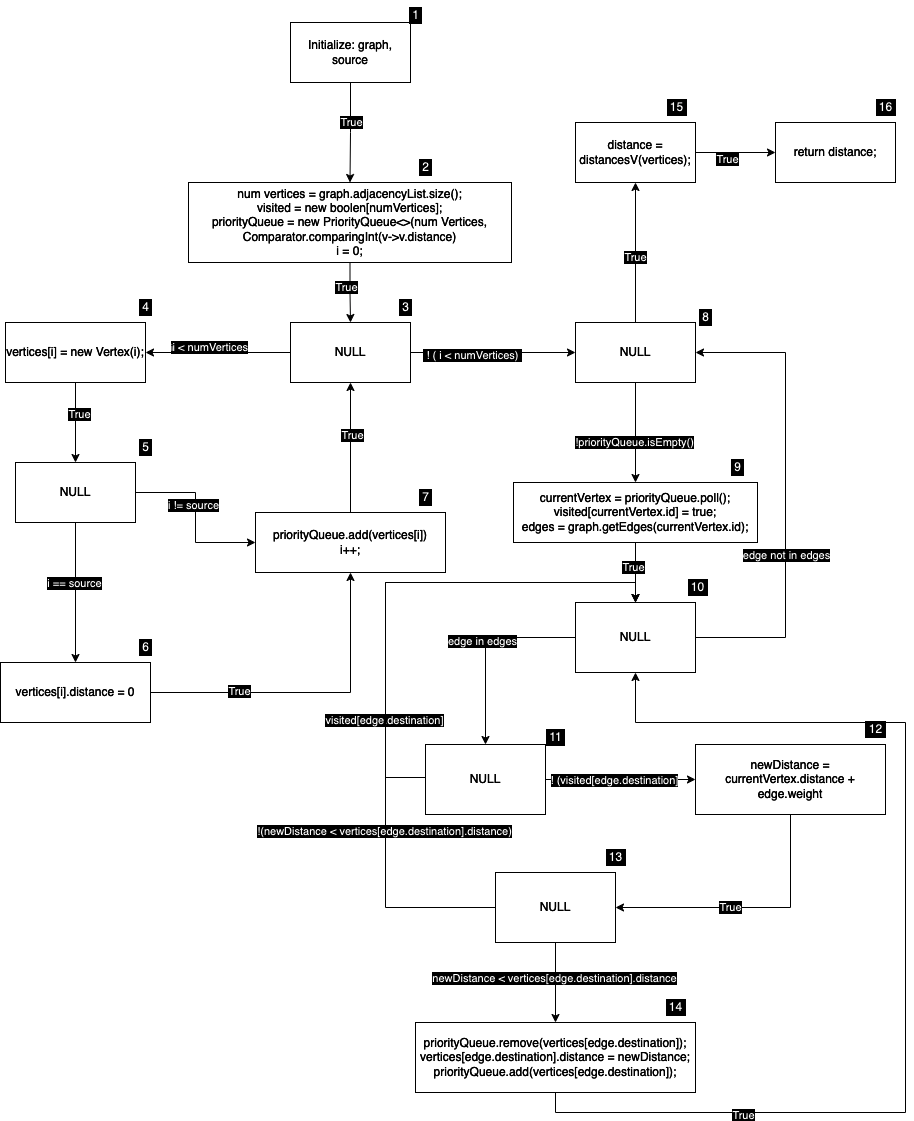
\includegraphics[width=\textwidth]{Images/DataFlowDijkstra.png}
    \caption{Data Flow - função Dijkstra.} 
    \label{fig:DataFlow-Dijkstra}

    \end{figure}
    
    \item \textbf{Caminhos ADUP}\\
    \texttt{}\par Para cada variável, iremos identificar caminhos no gráfico de fluxo de dados que satisfaçam os critérios de seleção (todos os caminhos du
para cada variável).\\
    O nó \textbf{1} corresponde ao Start, e o nó \textbf{16} corresponde ao End.
    Nesta função, as variáveis são as seguintes:\\
    \textit{graph}, \textit{visited}, \textit{numVertices}, \textit{priorityQueue}, \textit{newDistance}, \textit{distance}, \textit{source}, \textit{currentVertex}, \textit{edges}, \textit{vertices} e \textit{i}.
    \begin{itemize}
        \item \textbf{graph - global}
        \begin{itemize}
            \item ADUP1 - 1,2
            \item ADUP2 - 1, 2, 3, 8, 9
            \item ADUP3 - 1, 2, 3, 4, 5, 7, 3, 8, 9
            \item ADUP4 - 1, 2, 3, 4, 5, 6, 7, 3, 8, 9
            \item Caminho completo: 1, 2, 3, 4, 5, 6, 7, 3, 9, 10, 11, 12, 13, 14, 10, 15, 16
        \end{itemize}
        \item \textbf{visited}
        \begin{itemize}
            \item ADUP1 - 2, 3, 8, 9
            \item ADUP2 - 2, 3, 4, 5, 7, 3, 8, 9
            \item ADUP3 - 2, 3, 4, 5, 6, 7, 3, 8, 9
            \item ADUP4 - 9, 10, 11, 10
            \item ADUP5 - 9, 10, 11, 12
    
            \item Caminho completo: 1, 2, 3, 4, 5, 6, 7, 3, 9, 10, 11, 12, 13, 14, 10, 15, 16
        \end{itemize}
        \item \textbf{numVertices}
        \begin{itemize}
            \item ADUP1 - 2, 3, 4
            \item ADUP2 - 2, 3, 8
            \item Caminho completo: 1, 2, 3, 4, 5, 7, 3, 8, 9, 10, 15, 16
        \end{itemize}
        \item \textbf{priorityQueue}
        \begin{itemize}
            \item ADUP1 - 2, 3, 4, 5, 7
            \item ADUP2 - 2, 3, 4, 5, 6, 7
            \item ADUP3 - 7, 3, 8, 15
            \item ADUP4 - 7, 3, 8, 9
            \item ADUP5 - 9, 10, 11, 12, 13, 14
            \item Caminho completo:  1, 2, 3, 4, 5, 6, 7, 3, 9, 10, 11, 12, 13, 14, 10, 15, 16
        \end{itemize}
        NOTA: priorityQueue.poll() é uma definição pois remove o primeiro elemento da fila.
        \item \textbf{newDistance}
        \begin{itemize}
            \item ADUP1 - 12, 13, 14
            \item ADUP2 - 12, 13, 10
            \item Caminho completo: 1, 2, 3, 4, 5, 6, 7, 3, 9, 10, 11, 12, 13, 14, 10, 15, 16
        \end{itemize}
        \item \textbf{distance}
        \begin{itemize}
            \item ADUP1 - 15, 16
            \item Caminho completo: 1, 2, 3, 4, 5, 6, 7, 3, 9, 10, 11, 12, 13, 14, 10, 15, 16
        \end{itemize}
        \item \textbf{source - global}
        \begin{itemize}
            \item ADUP1 - 1, 2, 3, 4, 5, 7
            \item ADUP2 - 1, 2, 3, 4, 5, 6
            \item Caminho completo: 1, 2, 3, 4, 5, 6, 7, 3, 9, 10, 11, 12, 13, 14, 10, 15, 16
        \end{itemize}
        \item \textbf{currentVertex}
        \begin{itemize}
            \item ADUP1 - 9, 10, 11, 12
            \item Caminho completo: 1, 2, 3, 4, 5, 6, 7, 3, 9, 10, 11, 12, 13, 14, 10, 15, 16
        \end{itemize}
        \item \textbf{edge}
        \begin{itemize}
            \item ADUP1 - 9, 10, 8
            \item ADUP2 - 9, 10, 11
            \item Caminho completo: 1, 2, 3, 4, 5, 6, 7, 3, 9, 10, 11, 12, 13, 14, 10, 15, 16
        \end{itemize}
        \item \textbf{edge}
        \begin{itemize}
            \item ADUP1 - 9, 10, 11
            \item ADUP2 - 9, 10, 8
            \item ADUP3 - 9, 10, 11, 12
            \item ADUP4 - 9, 10, 11, 10
            \item ADUP5 - 9, 10, 11, 12, 13, 14
            \item ADUP6 - 9, 10, 11, 12, 13, 10
            \item Caminho completo: 1, 2, 3, 4, 5, 6, 7, 3, 9, 10, 11, 12, 13, 14, 10, 15, 16
        \end{itemize}
        \item \textbf{vertices}
        \begin{itemize}
            \item ADUP1 - 2, 3, 4
            \item ADUP2 - 4, 5, 6
            \item ADUP3 - 4, 5, 7
            \item ADUP4 - 6, 7
            \item ADUP5 - 4, 5, 7, 3, 8, 15
            \item ADUP6 - 4, 5, 7, 3, 8, 9, 10, 11, 12, 13, 10
            \item ADUP7 - 4, 5, 7, 3, 8, 9, 10, 11, 12, 13, 14
            \item ADUP8 - 6, 7, 3, 8, 15
            \item ADUP9 - 6, 7, 3, 8, 9, 10, 11, 12, 13, 10
            \item ADUP10 - 6, 7, 3, 8, 9, 10, 11, 12, 13, 14
            \item Caminho completo: 1, 2, 3, 4, 5, 6, 7, 3, 9, 10, 11, 12, 13, 14, 10, 15, 16
        \end{itemize}
        \item \textbf{i}
        \begin{itemize}
            \item ADUP1 - 2, 3
            \item ADUP2 - 2, 3, 4
            \item ADUP3 - 2, 3, 4, 5, 7
            \item ADUP4 - 2, 3, 4, 5, 6, 7
            \item ADUP5 - 7, 3
            \item ADUP6 - 7, 3, 4, 5
            \item ADUP7 - 7, 3, 4, 5, 6
            \item Caminho completo: 1, 2, 3, 4, 5, 6, 7, 3, 9, 10, 11, 12, 13, 14, 10, 15, 16
        \end{itemize}
      
    \end{itemize}

    Iremos apresentar de seguida os casos de teste para os caminhos completos acima descritos.\\

    \item \textbf{Casos de teste - Data Flow}\\
    Para a tabela ficar mais visível iremos apresentar os dois caminhos que conseguem passar pelos casos de teste.\\
    \begin{itemize}
        \item \textbf{PATH1} - 1, 2, 3, 4, 5, 6, 7, 3, 9, 10, 11, 12, 13, 14, 10, 15, 16
        \item \textbf{PATH2} - 1, 2, 3, 4, 5, 7, 3, 8, 9, 10, 15, 16
    \end{itemize}
    Os inputs são:\\
    \begin{itemize}
        \item \textbf{INPUT1}:\\\newline int numVertices = 5;\newline
        Graph graph = new Graph(numVertices);\newline
        graph.addEdge(0,2,1);\newline
                graph.addEdge(0,1,10);\newline
                graph.addEdge(2,4,5);\newline
                graph.addEdge(2,3,10);\newline
                graph.addEdge(3,4,3);\newline
                int[][] distance = dijkstra(graph, 0);

        \item \textbf{INPUT2}:\\\newline int numVertices = 1;\newline
        Graph graph = new Graph(numVertices);\newline
        int[][] distance = dijkstra(graph, 1);
    \end{itemize}

    \begin{table}[H]
        \centering
        \begin{tabular}{|c|c|c|p{4cm}|c|} % Ajusta a largura da coluna "Input" para 5cm
        \hline
        \textbf{variável} & \textbf{Caso de teste} & \textbf{Caminho} & \textbf{Graph} & \textbf{Source} \\ \hline
        graph & CT01 & PATH1  & INPUT1 &  0\\ \hline
        visited & CT02 & PATH1 & INPUT1 &  0  \\ \hline
        numVertices & CT03 & PATH2 &  INPUT2 &  1  \\ \hline
        priorityQueue & CT04 & PATH1  & INPUT1 &  0  \\ \hline
        newDistance & CT05 & PATH1 &  INPUT1 &  0  \\ \hline
        distance & CT06 &  PATH1  &  INPUT1 &  0  \\ \hline
        source & CT07 &    PATH1 & INPUT1 &  0 \\ \hline
        currentVertex & CT08  &PATH1 &  INPUT1 &  0 \\ \hline
        edges & CT09 & PATH1 &   INPUT1 &  0 \\ \hline
        vertices & CT10 & PATH1 &  INPUT1 &  0 \\ \hline
        i & CT11 & PATH1 &  INPUT1 &  0  \\ 

        \hline
    \end{tabular}
    \caption{Casos de teste para os caminhos ADUP do Dijkstra.}
    \label{tab:tabela_exemplo}
\end{table}
\clearpage
\end{enumerate}
    \item\textbf{Função Solve()}
    
       
    \begin{enumerate}
        
        \item \textbf{Grafo de Data Flow}
    \begin{figure}[H]
    \centering
    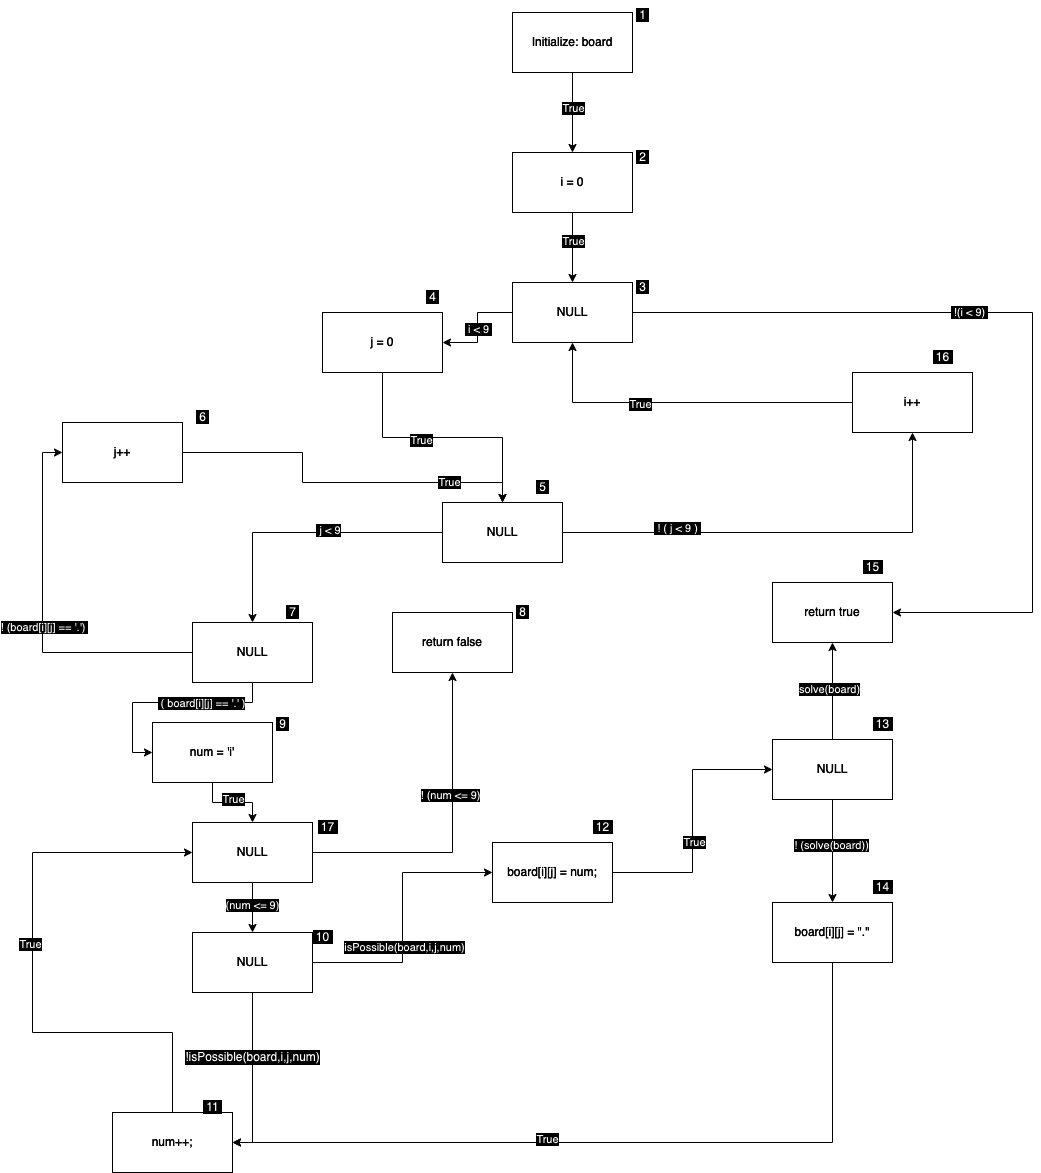
\includegraphics[width=\textwidth]{Images/DataFlowSudoku.png}
    \caption{Data Flow - função Solve.} 
    \label{fig:DataFlow-Solve}

    \end{figure}
    \item \textbf{Caminhos ADUP}\\
    
    Para cada variável, iremos identificar caminhos no gráfico de fluxo de dados que satisfaçam os critérios de seleção (todos os caminhos du
para cada variável).
O nó \textbf{1} corresponde ao Start, e os nós \textbf{8}, \textbf{15} correspondem ao End.
    Nesta função, as variáveis são as seguinte:\\
    \textit{board}, \textit{i}, \textit{j}, \textit{num}.
    \begin{itemize}
        \item \textbf{board - global }
        \begin{itemize}
            \item ADUP1 - 1, 2, 4, 3, 5, 7, 6
            \item ADUP2 - 1, 2, 4, 3, 5, 7, 9
            \item ADUP2 - 1, 2, 3, 5, 7, 9, 17, 10, 12
            \item ADUP3 - 1, 2, 3, 5, 7, 9, 17, 10, 11
            \item ADUP4 - 12, 13, 15
            \item ADUP5 - 12, 13, 14, 11, 17, 10, 11
            \item ADUP6 - 12, 13, 14, 11, 17, 10, 12

            \item Caminho completo: 1, 2, 3, 4, 5, 7, 9, 17, 10, 11, 17, 10, 12, 13, 14, 11, 17, 8. e
            1, 2, 3, 4, 5, 7, 6, 5, 16, 3, 4, 5, 7, 6, 5, 7, 9, 10, 11, 10, 12, 13, 15\newline
           NOTA: São necessários 2 caminhos para completar todos os nós.\newline
        \end{itemize}
        \item \textbf{i}
        \begin{itemize}
            \item ADUP1 - 2, 3,15
            \item ADUP2 - 2, 3, 4
            \item ADUP3 - 2, 3, 4, 5, 7, 6
            \item ADUP4 - 2, 3, 4, 5, 7, 9
            \item ADUP5 - 2, 3, 4, 5, 16
            \item ADUP6 - 2, 3, 4, 5, 7, 9, 17, 8
            \item ADUP7 - 2, 3, 4, 5, 7, 9, 17, 10, 11
            \item ADUP8 - 2, 3, 4, 5, 7, 9, 17, 10, 12
            \item ADUP9 - 2, 3, 4, 5, 7, 9, 17, 10, 13, 14
            \item ADUP10 - 16, 3, 4
            \item ADUP11 - 16, 3, 15
            \item ADUP12 - 16, 3, 4, 5, 7, 6
            \item ADUP13 - 16, 3, 4, 5, 7, 9
            \item ADUP14 - 16, 3, 4, 5, 16
            \item ADUP15 - 16, 3, 4, 5, 7, 9, 17, 8
            \item ADUP16 - 16, 3, 4, 5, 7, 9, 17, 10, 11
            \item ADUP17 - 16, 3, 4, 5, 7, 9, 17, 10, 12
            \item Caminho completo: 1, 2, 3, 4, 5, 7, 9, 17, 10, 11, 17, 10, 12, 13, 14, 11, 17, 8. e
            1, 2, 3, 4, 5, 7, 6, 5, 16, 3, 4, 5, 7, 6, 5, 7, 9, 10, 11, 10, 12, 13, 15\newline
           NOTA: São necessários 2 caminhos para completar todos os nós.\newline
         \end{itemize}
        \item \textbf{j}
        \begin{itemize}
            \item ADUP1 - 4, 5, 16, 3,(4)
            \item ADUP2 - 4, 5, 7, 6 
            \item ADUP3 - 4, 5, 7, 9, 17, 8
            \item ADUP4 - 4, 5, 7, 9, 17, 10, 11
            \item ADUP5 - 4, 5, 7, 9, 17, 10, 12
            \item ADUP6 - 6, 5, 16, 3, 4
            \item ADUP7 - 6, 5, 7, (6)
            \item ADUP9 - 6, 5, 7, 9, 17, 10, 12
            \item ADUP10 - 6, 5, 7, 9, 17, 10, 12, 13, 14
            \item ADUP11 - 6, 5, 7, 9, 17, 10, 11
            \item Caminho completo: 1, 2, 3, 4, 5, 7, 9, 17, 10, 11, 17, 10, 12, 13, 14, 11, 17, 8. e
            1, 2, 3, 4, 5, 7, 6, 5, 16, 3, 4, 5, 7, 6, 5, 7, 9, 10, 11, 10, 12, 13, 15\newline
           NOTA: São necessários 2 caminhos para completar todos os nós.\newline
       \end{itemize}
        \item \textbf{num}
        \begin{itemize}
            \item ADUP1 - 9, 17, 8
            \item ADUP2 - 9, 17, 10
            \item ADUP3 - 9, 17, 10, 11
            \item ADUP4 - 9, 17, 10, 12
            \item ADUP5 - 11, 17, 10
            \item ADUP6- 11, 17, 8
            \item ADUP7 - 11, 17, 10, 12
            \item ADUP8 - 11, 17, 10, (11)
            \item Caminho completo: 1, 2, 3, 4, 5, 7, 9, 17, 10, 11, 17, 10, 12, 13, 14, 11, 17, 8. e
            1, 2, 3, 4, 5, 7, 6, 5, 16, 3, 4, 5, 7, 6, 5, 7, 9, 10, 11, 10, 12, 13, 15\newline
           NOTA: São necessários 2 caminhos para completar todos os nós.\newline
       \end{itemize}
    \end{itemize}
    \item \textbf{Casos de teste - Data Flow}\\
    
    Para a tabela ficar mais visível iremos apresentar os dois caminhos que conseguem passar pelos casos de teste.\\
    \begin{itemize}
        \item \textbf{PATH1} - 1, 2, 3, 4, 5, 7, 9, 17, 10, 11, 17, 10, 12, 13, 14, 11, 17, 8
        \item \textbf{PATH2} - 1, 2, 3, 4, 5, 7, 6, 5, 16, 3, 4, 5, 7, 6, 5, 7, 9, 10, 11, 10, 12, 13, 15
    \end{itemize}
    Os inputs são:\\
    \begin{itemize}
        \item \textbf{INPUT1}:\\\newline  {'.', '.', '4', '6', '7', '8', '9', '1', '2'},\newline
        {'.', '7', '2', '1', '9', '5', '3', '4', '8'},\newline
        {'1', '9', '8', '3', '4', '.', '5', '6', '7'},\newline
        {'8', '5', '.', '7', '6', '1', '4', '2', '3'},\newline
        {'2', '2', '6', '8', '5', '3', '.', '.', '1'},\newline
        {'7', '1', '3', '9', '2', '4', '8', '5', '6'},\newline
        {'9', '.', '1', '.', '3', '.', '2', '8', '4'},\newline
        {'.', '8', '7', '4', '1', '9', '6', '3', '5'},\newline
        {'3', '4', '5', '2', '.', '6', '1', '7', '9'}\newline

        \item \textbf{INPUT2}:\\\newline 
            {'5', '3', '4', '6', '7', '8', '9', '1', '2'},\newline
            {'6', '7', '2', '1', '9', '5', '3', '4', '8'},\newline
            {'1', '9', '8', '3', '4', '2', '5', '6', '7'},\newline
            {'8', '5', '9', '7', '6', '1', '4', '2', '3'},\newline
            {'4', '2', '6', '8', '5', '3', '7', '9', '1'},\newline
            {'7', '1', '3', '9', '2', '4', '8', '5', '6'},\newline
            {'9', '6', '1', '5', '3', '7', '2', '8', '4'},\newline
            {'2', '8', '7', '4', '1', '9', '6', '3', '5'},\newline
            {'3', '4', '5', '2', '8', '6', '1', '7', '.'}\newline
       
    \end{itemize}
    O caminho \textbf{PATH1} e \textbf{PATH2} correspondem respetivamente ao \textbf{INPUT1} e \textbf{INPUT2}.
    
    \begin{table}[H]
        \centering
        \begin{tabular}{|c|c|c|p{4cm}|c|} % Ajusta a largura da coluna "Input" para 5cm
        \hline
        \textbf{Variável} & \textbf{Caso de teste} & \textbf{Caminho} & \textbf{Input} \\ \hline
        board & CT01 & PATH1 e PATH2 & INPUT1 e INPUT2    \\ \hline
        i & CT02 & PATH1 e PATH2 & INPUT1 e INPUT2   \\ \hline
        j & CT03 & PATH1 e PATH2 & INPUT1 e INPUT2   \\ \hline
        num & CT04 &  PATH1 e PATH2 & INPUT1 e INPUT2   \\ 
        \hline
    \end{tabular}
    \caption{Casos de teste para os caminhos ADUP do Sudoku.}
    \label{tab:tabela_exemplo}
\end{table}
    
    \end{enumerate}

    
\end{itemize}



\section{Critérios de Pass/Fail}

\texttt{}\par Testes unitários são uma prática essencial no desenvolvimento de software que tem como objetivo garantir a qualidade e a robustez do código. Estes consistem na verificação individual e isolada de unidades de código tais como funções, garantindo que cada unidade funcione conforme o esperado.

Portanto, para este tipo de teste, só é considerado bem sucedido se o output corresponder ao output esperado.

Se todos os testes forem sucedidos com sucesso, podemos dizer que o software funciona conforme planejado.
\section{Entregáveis de testes}
\begin{itemize}
    \item problem.txt - Apresenta a funcionalidade do software escolhido para testar.
    \item Diagramas: as pastas DataFlow e ControlFlow contêm os seus diagramas correspondentes de cada técnica.
    \item Código:
    \begin{itemize}
        \item \textbf{code.java} - contêm o código da resolução do Sudoku. Que é o código fonte do software que testamos.
        \item \textbf{dijkstra.java} - contêm o código da resolução do Sudoku. Que é o código fonte do software que testamos.
    \end{itemize}
    \item Outputs - Esta pasta contém todos os outputs esperados e os outputs finais.
    \item Relatório:
    \begin{itemize}
        \item Plano de testes.
        \item Casos de teste.
        \item Ambiente necessário para o teste de white box.
        \item Critérios de teste.
        \item Conclusão de teste.
    \end{itemize}
\end{itemize}

\section{Necessidades do ambiente}

\texttt{}\par É necessário usar um IDE, foi utilizado o VS code.

O uso da ferramenta diff é recomendado para que se possa comparar os outputs esprados com os finais.

Para testagem de inputs, é necessário ter o Java instalado.

Para executar é necessário, ter a terminologia " \textgreater{} ", por exemplo, na linha de comando:\\

/openjdk-21.0.2/Contents/Home/bin/java Code.Dijkstra \textgreater{} Outputs/ControlFlow/Output/Dijkstra/P5.txt\\

Isto significa, executar o software e o output ir para o file P5.txt. O input tem de ser colocado previamente.

\section{Divisão de tarefas}

\texttt{}\par Cada elemento do grupo ficou responsável por uma função, neste caso o Bruno ficou responsável pela função \textit{Dijkstra}, e o Rui pela função \textit{Solve}.\\

Sendo que ao longo do desenvolvimento, fomos nos ajudando um ao outro, realizando o debate dos planos de tstes, a implementação do caminhos, a realização do data flow.


\clearpage
\section{Relatório de Conclusão dos Testes}
\texttt{}\par Nesta secção apresentamos os resultados dos testes unitários de acordo com o critério de Pass/Fail definidos na secção 6.
\subsection{Control Flow Testing}
\begin{table}[H]
    \centering
    \renewcommand{\arraystretch}{1.8}
    \begin{tabular}{|c|p{4cm}|p{4cm}|c|c|} % Ajusta a largura da coluna "Input" para 5cm
    \hline 
    \textbf{Teste} & \textbf{Output Esperado} & \textbf{Output} & \textbf{Comentário} & \textbf{Passou/Falhou}\\
    \hline

    \textbf{P3}  & 0 - 2147483647  & 0 - 2147483647 & Ok & \cellcolor{green}  \\
    \hline
    \textbf{P4} & 0 - 0 & 0 - 0 & Ok & \cellcolor{green}  \\
    \hline
    \textbf{P5}  & 0 - 0\newline
    1 - 2147483647\newline
    2 - 2147483647\newline
    3 - 2147483647\newline
    4 - 2147483647    & 0 - 0\newline
    1 - 2147483647\newline
    2 - 2147483647\newline
    3 - 2147483647\newline
    4 - 2147483647    & Ok & \cellcolor{green}  \\
    \hline
    \textbf{P6}   & 0 - 0\newline
    1 - 2147483647  & 0 - 0\newline
    1 - 2147483647   & Ok & \cellcolor{green}  \\
    \hline
    \textbf{P7}  & 0 - 0\newline
    1 - 10\newline
    2 - 1\newline
    3 - 11\newline
    4 - 6   & 0 - 0\newline
    1 - 10\newline
    2 - 1\newline
    3 - 11\newline
    4 - 6  & Ok & \cellcolor{green}  \\
    \hline

\end{tabular}
\caption{Resultados para os casos de teste da função de Dijkstra.}
\label{tab:tabela_exemplo}
\end{table}
De acordo com a seção 6, o software atende aos critérios. (100\% sucesso).






\begin{table}[H]
    \centering
    \renewcommand{\arraystretch}{1.2}
    \begin{tabular}{|c|p{4cm}|p{4cm}|c|c|} % Ajusta a largura da coluna "Input" para 5cm
    \hline
    \textbf{Teste} & \textbf{Output Esperado} & \textbf{Output} & \textbf{Comentário} & \textbf{Passou/Falhou}\\
    \hline
    \textbf{P2} &   
    5 3 4 6 7 8 9 1 2 \newline
    6 7 2 1 9 5 3 4 8 \newline
    1 9 8 3 4 2 5 6 7 \newline
    8 5 9 7 6 1 4 2 3 \newline
    4 2 6 8 5 3 7 9 1 \newline
    7 1 3 9 2 4 8 5 6 \newline
    9 6 1 5 3 7 2 8 4 \newline
    2 8 7 4 1 9 6 3 5 \newline
    3 4 5 2 8 6 1 7 9 & 
5 3 4 6 7 8 9 1 2 \newline
6 7 2 1 9 5 3 4 8 \newline
1 9 8 3 4 2 5 6 7 \newline  
8 5 9 7 6 1 4 2 3 \newline
4 2 6 8 5 3 7 9 1 \newline
7 1 3 9 2 4 8 5 6 \newline
9 6 1 5 3 7 2 8 4 \newline
2 8 7 4 1 9 6 3 5 \newline
3 4 5 2 8 6 1 7 9   & Ok & \cellcolor{green}  \\
\hline
\textbf{P3} & 
4 5 6 7 8 9 1 2 3\newline
7 8 9 1 2 3 4 5 6\newline
2 1 4 3 6 5 8 9 7\newline
3 6 5 8 9 7 2 1 4 \newline
8 9 7 2 1 4 3 6 5\newline
5 3 1 6 4 2 9 7 8\newline
6 4 2 9 7 8 5 3 1\newline
9 7 8 5 3 1 6 4 2 
 & 1 2 3 4 5 6 7 8 9\newline
4 5 6 7 8 9 1 2 3\newline
7 8 9 1 2 3 4 5 6\newline
2 1 4 3 6 5 8 9 7\newline
3 6 5 8 9 7 2 1 4 \newline
8 9 7 2 1 4 3 6 5\newline
5 3 1 6 4 2 9 7 8\newline
6 4 2 9 7 8 5 3 1\newline
9 7 8 5 3 1 6 4 2 & Ok & \cellcolor{green}  \\
\hline
\textbf{P4} &  
. 3 4 5 7 8 9 1 2 \newline
6 7 2 1 9 5 3 4 8 \newline
1 9 8 3 4 2 5 6 7 \newline
8 5 9 7 6 1 4 2 3 \newline
4 2 6 8 5 3 7 9 1 \newline
7 1 3 9 2 4 8 5 6 \newline
9 6 1 5 3 7 2 8 4 \newline
2 8 7 4 1 9 6 3 5 \newline
3 4 5 2 8 6 1 7 9   
 & 
    . 3 4 5 7 8 9 1 2 \newline
    6 7 2 1 9 5 3 4 8 \newline
    1 9 8 3 4 2 5 6 7 \newline
    8 5 9 7 6 1 4 2 3 \newline
    4 2 6 8 5 3 7 9 1 \newline
    7 1 3 9 2 4 8 5 6 \newline
    9 6 1 5 3 7 2 8 4 \newline
    2 8 7 4 1 9 6 3 5 \newline
    3 4 5 2 8 6 1 7 9   & Ok & \cellcolor{green}  \\
\hline

\textbf{P5} &  . . 4 6 7 8 9 1 2 \newline
. 7 2 1 9 5 3 4 8 \newline
1 9 8 3 4 . 5 6 7 \newline
8 5 . 7 6 1 4 2 3 \newline
2 2 6 8 5 3 . . 1 \newline
7 1 3 9 2 4 8 5 6 \newline
9 . 1 . 3 . 2 8 4 \newline
. 8 7 4 1 9 6 3 5 \newline
3 4 5 2 . 6 1 7 9 
 & . . 4 6 7 8 9 1 2 \newline
. 7 2 1 9 5 3 4 8 \newline
1 9 8 3 4 . 5 6 7 \newline
8 5 . 7 6 1 4 2 3 \newline
2 2 6 8 5 3 . . 1 \newline
7 1 3 9 2 4 8 5 6 \newline
9 . 1 . 3 . 2 8 4 \newline
. 8 7 4 1 9 6 3 5 \newline
3 4 5 2 . 6 1 7 9 & Ok & \cellcolor{green}  \\
\hline
\textbf{P6} & 
5 3 4 6 7 8 9 1 2 \newline
6 7 2 1 9 5 3 4 8\newline
1 9 8 3 4 2 5 6 7\newline
8 5 9 7 6 1 4 2 3\newline
4 2 6 8 5 3 7 9 1\newline
7 1 3 9 2 4 8 5 6\newline
9 6 1 5 3 7 2 8 4\newline
2 8 7 4 1 9 6 3 5\newline
3 4 5 2 8 6 1 7 9 &
    5 3 4 6 7 8 9 1 2 \newline
6 7 2 1 9 5 3 4 8\newline
1 9 8 3 4 2 5 6 7\newline
8 5 9 7 6 1 4 2 3\newline
4 2 6 8 5 3 7 9 1\newline
7 1 3 9 2 4 8 5 6\newline
9 6 1 5 3 7 2 8 4\newline
2 8 7 4 1 9 6 3 5\newline
3 4 5 2 8 6 1 7 9 & Ok & \cellcolor{green}  \\
\hline
\end{tabular}
\caption{Resultados para os casos de teste da função de Solve.}
\label{tab:tabela_exemplo}
\end{table}


\subsection{Data Flow Testing}

\begin{table}[H]
    \centering
    \renewcommand{\arraystretch}{1.1}
    \begin{tabular}{|c|p{4cm}|p{4cm}|c|c|} % Ajusta a largura da coluna "Input" para 5cm
    \hline
    \textbf{Teste} & \textbf{Output Esperado} & \textbf{Output} & \textbf{Comentário} & \textbf{Passou/Falhou}\\ \hline
    CT01 &0 - 0
    1 - 10 \newline
    2 - 1 \newline
    3 - 11 \newline
    4 - 6  & 0 - 0
    1 - 10 \newline
    2 - 1 \newline
    3 - 11 \newline
    4 - 6  & Ok & \cellcolor{green} \\  \hline
    CT02 &0 - 0
    1 - 10 \newline
    2 - 1 \newline
    3 - 11 \newline
    4 - 6  & 0 - 0
    1 - 10 \newline
    2 - 1 \newline
    3 - 11 \newline
    4 - 6  & Ok & \cellcolor{green} \\  \hline
    CT03 & 0 - 2147483647 & 0 - 2147483647 & Ok &  \cellcolor{green}  \\ \hline
    CT04 &0 - 0
    1 - 10 \newline
    2 - 1 \newline
    3 - 11 \newline
    4 - 6  & 0 - 0
    1 - 10 \newline
    2 - 1 \newline
    3 - 11 \newline
    4 - 6  & Ok &  \cellcolor{green} \\ \hline
    CT05 &0 - 0
    1 - 10 \newline
    2 - 1 \newline
    3 - 11 \newline
    4 - 6  & 0 - 0
    1 - 10 \newline
    2 - 1 \newline
    3 - 11 \newline
    4 - 6  & Ok & \cellcolor{green}  \\ \hline
    CT06 &0 - 0
    1 - 10 \newline
    2 - 1 \newline
    3 - 11 \newline
    4 - 6  & 0 - 0
    1 - 10 \newline
    2 - 1 \newline
    3 - 11 \newline
    4 - 6  & Ok & \cellcolor{green}  \\ \hline
    CT07 &0 - 0
    1 - 10 \newline
    2 - 1 \newline
    3 - 11 \newline
    4 - 6  & 0 - 0
    1 - 10 \newline
    2 - 1 \newline
    3 - 11 \newline
    4 - 6  & Ok &  \cellcolor{green} \\ \hline
    CT08 &0 - 0
    1 - 10 \newline
    2 - 1 \newline
    3 - 11 \newline
    4 - 6  & 0 - 0
    1 - 10 \newline
    2 - 1 \newline
    3 - 11 \newline
    4 - 6  & Ok &  \cellcolor{green} \\ \hline
    CT09 &0 - 0
    1 - 10 \newline
    2 - 1 \newline
    3 - 11 \newline
    4 - 6  & 0 - 0
    1 - 10 \newline
    2 - 1 \newline
    3 - 11 \newline
    4 - 6  & Ok &  \cellcolor{green} \\ \hline
    CT10 &0 - 0
    1 - 10 \newline
    2 - 1 \newline
    3 - 11 \newline
    4 - 6  & 0 - 0
    1 - 10 \newline
    2 - 1 \newline
    3 - 11 \newline
    4 - 6  & Ok &  \cellcolor{green} \\ \hline
    CT11 &0 - 0
    1 - 10 \newline
    2 - 1 \newline
    3 - 11 \newline
    4 - 6  & 0 - 0
    1 - 10 \newline
    2 - 1 \newline
    3 - 11 \newline
    4 - 6  & Ok &  \cellcolor{green}  \\ \hline



\end{tabular}
\caption{Resultados para os casos de teste da função de Dijkstra.}
\label{tab:tabela_exemplo}
\end{table}




Nesta tabela, temos 2 inputs para cada teste, visto que para que o data flow fosse concluído com sucesso, era necessário passar por todos os caminhos, sendo que é não existe um caminho que passe por todos. Iremos seguir a ordem \textbf{INPUT1} e \textbf{INPUT2}.

\begin{table}[H]
    \centering
    \renewcommand{\arraystretch}{1.1}
    \begin{tabular}{|c|p{4cm}|p{4cm}|c|c|} % Ajusta a largura da coluna "Input" para 5cm
    \hline
    \textbf{Teste} & \textbf{Output Esperado} & \textbf{Output} & \textbf{Comentário} & \textbf{Passou/Falhou}\\ \hline
    CT01 & . . 4 6 7 8 9 1 2 \newline
    . 7 2 1 9 5 3 4 8 \newline
    1 9 8 3 4 . 5 6 7 \newline
    8 5 . 7 6 1 4 2 3 \newline
    2 2 6 8 5 3 . . 1 \newline
    7 1 3 9 2 4 8 5 6 \newline
    9 . 1 . 3 . 2 8 4 \newline
    . 8 7 4 1 9 6 3 5 \newline
    3 4 5 2 . 6 1 7 9 & . . 4 6 7 8 9 1 2 \newline
    . 7 2 1 9 5 3 4 8 \newline
    1 9 8 3 4 . 5 6 7 \newline
    8 5 . 7 6 1 4 2 3 \newline
    2 2 6 8 5 3 . . 1 \newline
    7 1 3 9 2 4 8 5 6 \newline
    9 . 1 . 3 . 2 8 4 \newline
    . 8 7 4 1 9 6 3 5 \newline
    3 4 5 2 . 6 1 7 9 & Ok & \cellcolor{green} \\ \hline


    CT02 & . . 4 6 7 8 9 1 2 \newline
    . 7 2 1 9 5 3 4 8 \newline
    1 9 8 3 4 . 5 6 7 \newline
    8 5 . 7 6 1 4 2 3 \newline
    2 2 6 8 5 3 . . 1 \newline
    7 1 3 9 2 4 8 5 6 \newline
    9 . 1 . 3 . 2 8 4 \newline
    . 8 7 4 1 9 6 3 5 \newline
    3 4 5 2 . 6 1 7 9 & . . 4 6 7 8 9 1 2 \newline
    . 7 2 1 9 5 3 4 8 \newline
    1 9 8 3 4 . 5 6 7 \newline
    8 5 . 7 6 1 4 2 3 \newline
    2 2 6 8 5 3 . . 1 \newline
    7 1 3 9 2 4 8 5 6 \newline
    9 . 1 . 3 . 2 8 4 \newline
    . 8 7 4 1 9 6 3 5 \newline
    3 4 5 2 . 6 1 7 9 & Ok & \cellcolor{green} \\ \hline

    CT03 & . . 4 6 7 8 9 1 2 \newline
    . 7 2 1 9 5 3 4 8 \newline
    1 9 8 3 4 . 5 6 7 \newline
    8 5 . 7 6 1 4 2 3 \newline
    2 2 6 8 5 3 . . 1 \newline
    7 1 3 9 2 4 8 5 6 \newline
    9 . 1 . 3 . 2 8 4 \newline
    . 8 7 4 1 9 6 3 5 \newline
    3 4 5 2 . 6 1 7 9 & . . 4 6 7 8 9 1 2 \newline
    . 7 2 1 9 5 3 4 8 \newline
    1 9 8 3 4 . 5 6 7 \newline
    8 5 . 7 6 1 4 2 3 \newline
    2 2 6 8 5 3 . . 1 \newline
    7 1 3 9 2 4 8 5 6 \newline
    9 . 1 . 3 . 2 8 4 \newline
    . 8 7 4 1 9 6 3 5 \newline
    3 4 5 2 . 6 1 7 9 & Ok & \cellcolor{green} \\ \hline

    CT04 & . . 4 6 7 8 9 1 2 \newline
    . 7 2 1 9 5 3 4 8 \newline
    1 9 8 3 4 . 5 6 7 \newline
    8 5 . 7 6 1 4 2 3 \newline
    2 2 6 8 5 3 . . 1 \newline
    7 1 3 9 2 4 8 5 6 \newline
    9 . 1 . 3 . 2 8 4 \newline
    . 8 7 4 1 9 6 3 5 \newline
    3 4 5 2 . 6 1 7 9 & . . 4 6 7 8 9 1 2 \newline
    . 7 2 1 9 5 3 4 8 \newline
    1 9 8 3 4 . 5 6 7 \newline
    8 5 . 7 6 1 4 2 3 \newline
    2 2 6 8 5 3 . . 1 \newline
    7 1 3 9 2 4 8 5 6 \newline
    9 . 1 . 3 . 2 8 4 \newline
    . 8 7 4 1 9 6 3 5 \newline
    3 4 5 2 . 6 1 7 9 & Ok & \cellcolor{green} \\ \hline
   

\end{tabular}
\caption{Resultados para o INPUT1 dataflow dos casos de teste da função de Solve.}
\label{tab:tabela_exemplo}
\end{table}


\begin{table}[H]
    \centering
    \renewcommand{\arraystretch}{1.1}
    \begin{tabular}{|c|p{4cm}|p{4cm}|c|c|} % Ajusta a largura da coluna "Input" para 5cm
    \hline
    \textbf{Teste} & \textbf{Output Esperado} & \textbf{Output} & \textbf{Comentário} & \textbf{Passou/Falhou}\\ \hline
    CT01 & 5 3 4 6 7 8 9 1 2 \newline
    6 7 2 1 9 5 3 4 8 \newline
    1 9 8 3 4 2 5 6 7 \newline
    8 5 9 7 6 1 4 2 3 \newline
    4 2 6 8 5 3 7 9 1 \newline
    7 1 3 9 2 4 8 5 6 \newline
    9 6 1 5 3 7 2 8 4 \newline
    2 8 7 4 1 9 6 3 5 \newline
    3 4 5 2 8 6 1 7 9  & 5 3 4 6 7 8 9 1 2 \newline
    6 7 2 1 9 5 3 4 8 \newline
    1 9 8 3 4 2 5 6 7 \newline
    8 5 9 7 6 1 4 2 3 \newline
    4 2 6 8 5 3 7 9 1 \newline
    7 1 3 9 2 4 8 5 6 \newline
    9 6 1 5 3 7 2 8 4 \newline
    2 8 7 4 1 9 6 3 5 \newline
    3 4 5 2 8 6 1 7 9  & Ok & \cellcolor{green} \\ \hline

    CT02 & 5 3 4 6 7 8 9 1 2 \newline
    6 7 2 1 9 5 3 4 8 \newline
    1 9 8 3 4 2 5 6 7 \newline
    8 5 9 7 6 1 4 2 3 \newline
    4 2 6 8 5 3 7 9 1 \newline
    7 1 3 9 2 4 8 5 6 \newline
    9 6 1 5 3 7 2 8 4 \newline
    2 8 7 4 1 9 6 3 5 \newline
    3 4 5 2 8 6 1 7 9  & 5 3 4 6 7 8 9 1 2 \newline
    6 7 2 1 9 5 3 4 8 \newline
    1 9 8 3 4 2 5 6 7 \newline
    8 5 9 7 6 1 4 2 3 \newline
    4 2 6 8 5 3 7 9 1 \newline
    7 1 3 9 2 4 8 5 6 \newline
    9 6 1 5 3 7 2 8 4 \newline
    2 8 7 4 1 9 6 3 5 \newline
    3 4 5 2 8 6 1 7 9  & Ok & \cellcolor{green} \\ \hline

    CT03 & 5 3 4 6 7 8 9 1 2 \newline
    6 7 2 1 9 5 3 4 8 \newline
    1 9 8 3 4 2 5 6 7 \newline
    8 5 9 7 6 1 4 2 3 \newline
    4 2 6 8 5 3 7 9 1 \newline
    7 1 3 9 2 4 8 5 6 \newline
    9 6 1 5 3 7 2 8 4 \newline
    2 8 7 4 1 9 6 3 5 \newline
    3 4 5 2 8 6 1 7 9  & 5 3 4 6 7 8 9 1 2 \newline
    6 7 2 1 9 5 3 4 8 \newline
    1 9 8 3 4 2 5 6 7 \newline
    8 5 9 7 6 1 4 2 3 \newline
    4 2 6 8 5 3 7 9 1 \newline
    7 1 3 9 2 4 8 5 6 \newline
    9 6 1 5 3 7 2 8 4 \newline
    2 8 7 4 1 9 6 3 5 \newline
    3 4 5 2 8 6 1 7 9  & Ok & \cellcolor{green} \\ \hline

    CT04 & 5 3 4 6 7 8 9 1 2 \newline
    6 7 2 1 9 5 3 4 8 \newline
    1 9 8 3 4 2 5 6 7 \newline
    8 5 9 7 6 1 4 2 3 \newline
    4 2 6 8 5 3 7 9 1 \newline
    7 1 3 9 2 4 8 5 6 \newline
    9 6 1 5 3 7 2 8 4 \newline
    2 8 7 4 1 9 6 3 5 \newline
    3 4 5 2 8 6 1 7 9  & 5 3 4 6 7 8 9 1 2 \newline
    6 7 2 1 9 5 3 4 8 \newline
    1 9 8 3 4 2 5 6 7 \newline
    8 5 9 7 6 1 4 2 3 \newline
    4 2 6 8 5 3 7 9 1 \newline
    7 1 3 9 2 4 8 5 6 \newline
    9 6 1 5 3 7 2 8 4 \newline
    2 8 7 4 1 9 6 3 5 \newline
    3 4 5 2 8 6 1 7 9  & Ok & \cellcolor{green} \\ \hline


\end{tabular}
\caption{Resultados para o INPUT2 dataflow dos casos de teste da função de Solve.}
\label{tab:tabela_exemplo}
\end{table}

\subsection{Análise de resultados}
Após visualização das tabelas podemos tirar boas conclusões, apartindo dos critérios apresentados na secção 6, ambos os softwares passam com 100\% de sucesso.

Todos os outputs recebidos eram os outputs esperados.

Analisamos e verificamos se com todos os testes realmente passavam pelos nós, e tiramos novos bons resultados. A cobertura do código é alta, tendo alguns testes com 100\% de cobertura. Estes resultados estão na pasta \textit{CodeCoverage}, em que apresetamos o code coverage para cada teste criado.

Os resultados obtidos nos testes unitários do DataFlow eram já esperados, visto que os testes são exatamente iguais aos do control flow.

\section{Conclusão}
\quad Durante este projeto, exploramos as técnicas de controlo de fluxo e fluxo de dados nos nossos testes unitários, focando especificamente na função \textit{Dijkstra} e \textit{Solve}. 

Ao aplicar o controlo de fluxo, pudemos examinar meticulosamente o comportamento do algoritmo em diferentes caminhos de execução, identificando áreas de código que exigiam atenção especial e garantindo uma cobertura abrangente dos casos de teste.

Da mesma forma, ao analisar o fluxo de dados, fomos capazes de rastrear como os dados eram manipulados e propagados ao longo do algoritmo.

Os resultados de nossa abordagem foram extremamente positivos.

Em suma, o controlo de fluxo e o fluxo de dados revelaram-se como ferramentas indispensáveis no nosso arsenal de testes unitários. Estamos confiantes de que continuaremos a aplicar e aprimorar essas técnicas nos nossos projetos futuros, garantindo assim a entrega de software de alta qualidade e confiabilidade.


\end{document}